\section{Results} \label{results}

\subsection{Evaluation Metrics}

Whereas the Mean Squared Error Loss was used for \emph{training} the Neural Network due to its convenient differentiability with regards to backpropagation, we preferred the Mean Absolute Error and the $R^2$ value for \emph{evaluating} the different models.
The MAE measures absolute deviations between true and predicted price and is therefore interpretable on the same scale as the original data.
While the $R^2$ certainly has some inherent flaws, it provides a scale-independent and highly interpretable measure of overall model fit.

When using the log-price for model fitting, all error metrics were computed on the \emph{original} price scale to obtain an interpretable MAE value.
More specifically, all computations were performed \emph{after} backtransforming the fitted values for the log-price to the raw price scale.
Since the results for the MAE and $R^2$ are highly dependent on the exact transformation procedure, they are in particular \emph{not comparable} with approaches that use a different evaluation strategy.

To illustrate this difference in more detail, denote the error metrics as functions of the true and predicted values:
%%%
\begin{align*}
  MAE(\mathbf{y}, \hat{\mathbf{y}})
   & = \frac{1}{n}\sum_{i = 1}^{n} \left| y_i - \hat{y}_i \right|                                               \\
  R^2(\mathbf{y}, \hat{\mathbf{y}})
   & = \frac{\sum_{i=1}^{n} \left( \hat{y}_i - \bar{y}\right)^2}{\sum_{i=1}^{n} \left( y_i - \bar{y} \right)^2}
\end{align*}
%%%
With this notation, we computed $MAE \left(\mathbf{y}, \exp \left(\widehat{\log(\mathbf{y})}\right)\right)$ which is of course not identical to $\exp \left(MAE \left(\log(\mathbf{y}), \widehat{\log(\mathbf{y})}\right) \right)$, i.e. backtransforming the error on the log-scale.
To stay consistent, we similarly computed $R^2 \left(\mathbf{y}, \exp \left(\widehat{\log(\mathbf{y})}\right)\right)$ on the original scale with the backtransformed fitted values instead of  $R^2 \left(\log(\mathbf{y}), \widehat{\log(\mathbf{y})}\right)$, where the latter usually leads to a better score.



\subsection{Predictive Performance}

%%%
\begin{figure}[t]
  \centering
  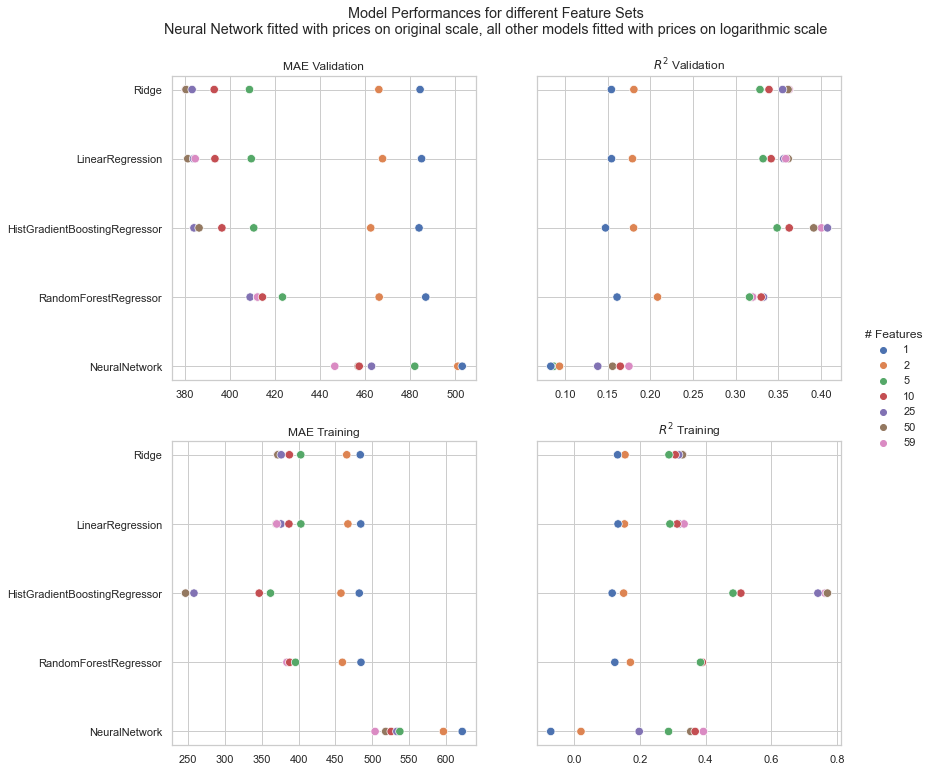
\includegraphics[width=\textwidth]{model_comparison.png}
  \caption{Performance Comparison of Classical Models with Neural Network}
  \label{fig:model-comparison}
\end{figure}
%%%

\Cref{fig:model-comparison} shows performance metrics for all fitted models on both, the training set and the validation set.
The different colors indicate how many features were selected by the \texttt{RFE} algorithm for this particular fit out of $59$ total predictor variables.
Unsurprisingly, one or two features (in case of the \texttt{RFE} the number of bedrooms and the (number of) accomodates) provide too little information to model the task appropriately.

However, including merely $5$ features (in this case adding the $30$ day availability, the indicator variable for the \emph{Frogner} neighbourhood and, notably, the price predictions from the Convolutional Net based on the image data) results in a very competitive performance for most models on the validation set.

The two subplots on the left display the MAE and tell a very similar story to the subplots on the right that show the $R^2$:
Generally, more features lead to better performance on training and validation set.
In case of the flexible Gradient Boosting algorithm and, to some minor extent, for the Random Forest, a high number of input features lead to \emph{overfitting} such that the performance on the training set is far superior to the values on out-of-sample data.
In contrast, models with few parameters such as Linear Regression or Ridge Regression generalize very well to the validation set with virtually no performance drop.

One exception to this rule is the highly complex Neural Network which appears to perform \emph{better} on out-of-sample data.
This phenomenon can be explained by the different behaviour of Dropout and Batchnorm layers in training and inference mode on the one hand and the presence of price outliers, which is discussed in \Cref{outliers}, on the other hand.

When comparing the models \emph{within} each subplot, all classical Machine Learning models perform similarly on the validation data.
This finding emphasizes two aspects:
%%%
\begin{enumerate}
  \item The prediction task does \textbf{not} require overly complex models and linear models perform just fine.
  \item We can expect predictions within a distance of roughly $400$ NOK (40 Euros) on average to the true price.
        Further, a $R^2$ value of around $0.4$ is the best we can hope for.
        These statements hold for fitting on the \emph{entire} training set, \Cref{outliers} reveals how the performance radically improves when excluding some observations.
\end{enumerate}
%%%
In comparison to all \texttt{scikit-learn} models, our custom Neural Net appears to underperform.
We have to keep in mind though, that evaluation on the validation set is overly optimistic for those models whose hyperparameters were tuned on this data during cross validation.
The best simulation of performance on truly unseen data is thus provided by the \emph{test} set that remained untouched up to this point.

\begin{table}[th]
  \centering
  \begin{tabular}{lrr}
    \hline
    Model                & \multicolumn{1}{c}{MAE} & \multicolumn{1}{c}{$R^2$} \\ \hline
    Linear Regression    & 404.709                 & 0.298                     \\
    Ridge                & 405.932                 & 0.294                     \\
    Random Forest        & 444.166                 & 0.268                     \\
    HistGradientBoosting & 412.243                 & 0.387                     \\
    Neural Network       & 402.24                  & 0.333                     \\
    Top2 Average         & 404.848                 & 0.296                     \\
    Top3 Average         & 399.315                 & 0.343                     \\
    Top4 Average         & 404.206                 & 0.332                     \\
    Top5 Average         & 408.116                 & 0.27                      \\ \hline
  \end{tabular}
  \caption{Test Set Performance of Classical Machine Learning Models, our custom Neural Network and Ensemble Predictions}
  \label{tab:test-set}
\end{table}

\Cref{tab:test-set} compares test set metrics for the best performing models on the validation set within each function class, i.e. the Neural Net version with all $59$ features and the Random Forest model with only $25$ features were selected.
In addition, we added some simple ensemble models that predict the average estimate from the top $2$, $3$, $4$ or all five models, respectively.

The Random Forest model indeed seems to have overfit on the validation set due to hyperparameter tuning, such that it now performs worst.
Quite surpringly, the Neural Net shows a significant performance boost on the test data and is now very competitive with all other models.
One plausible reason for this phenomenon is again related to outliers and explained in \Cref{outliers}.

Averaging predictions from multiple independent algorithms indicates promising results:
The Top $3$ ensemble achieves the lowest out-of-sample MAE of slightly below $400$ NOK.
As indicated by \Cref{fig:model-comparison} this particular ensemble averages the price predictions of the following three model configurations:
%%%
\begin{enumerate}
  \item Linear Regression with $50$ selected features.
  \item Ridge Regression with $50$ selected features and a penalty weight of $\alpha = 14$.
  \item Histogram Gradient Boosting Model with all $59$ features, a \emph{learning rate} of $0.09$, a \emph{maximum tree depth} of $18$, a \emph{maximum number of leaf nodes} within each tree of $30$ and a \emph{minimum number of samples} per leaf node of $4$.
\end{enumerate}
%%%




\subsection{Understanding and Interpretation}

Interpreting the results of high-dimensional and complex statistical models is notoriously difficult.
This section approaches the challenge from two opposite angles.

First, we reduce the \emph{complexity} by fitting a simple and well-understood Linear Regression model with the same features that were selected for the best-performing Neural Network and analyze the coefficients.

Second, we reduce the \emph{dimensionality} by leveraging a different Neural Network and visualize the results in two-dimensional space.

\subsubsection{Feature Importance}

One idea to draw conclusions about which features were most important for the Neural Network is to start with a random noise input and leverage Gradient information to optimize for new artificial inputs that maximally or minimally activate the output neuron, i.e. leading to very low or very high price predictions.
We chose a conceptually simpler approach and analyzed the feature importance of an auxiliary Linear Regression model instead based on the idea that important features for a simpler Linear Regression model might also be important for a more complex Neural Network.

Therefore we preselected $25$ of the network's input features with the \texttt{RFE} algorithm, which is introduced in \Cref{appendix:feature-selection}, and compared the coefficient \emph{magnitudes}.
As noted before, all predictors were standardized at the beginning of the data pipeline such that this comparison is meaningful.
The results are shown in \Cref{fig:coefficient-plot}.

\begin{figure}[t]
  \centering
  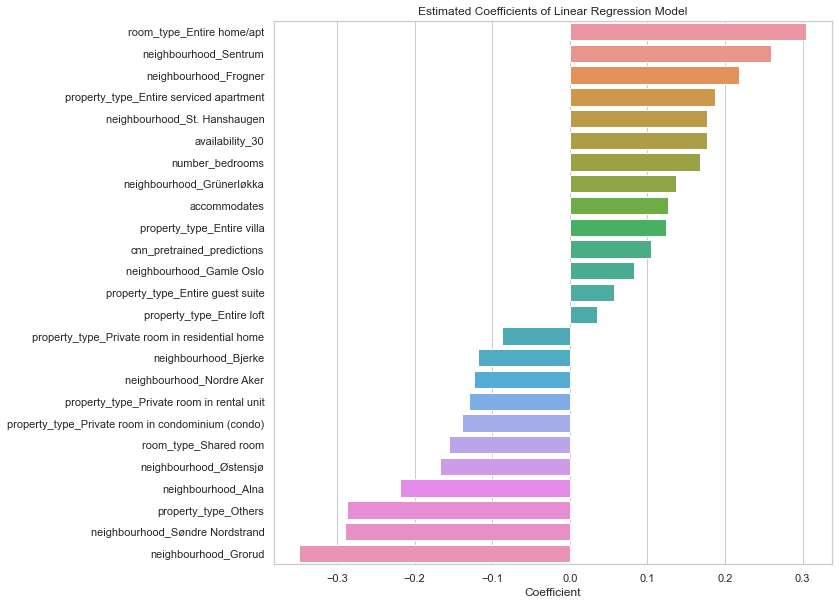
\includegraphics[width=0.8\textwidth]{coefficient_plot.png}
  \caption{Estimated coefficients of a Linear Regression model for $25$ preselected features}
  \label{fig:coefficient-plot}
\end{figure}

It is worth noting that the two most important features based on various different feature selectors within the \texttt{scikit-learn} library were always the number of \emph{bedrooms} and the (number of) \emph{accomodates} in this order, both measuring the apartment's \emph{capacity}.

The coefficient plot, however, is dominated by categorical features:
In agreement with human intuition, the \emph{room} type, the \emph{property} type and the \emph{neighbourhood} strongly influence the predicted price.
Unsurprisingly, the property types \emph{entire home} and \emph{entire villa} are connected with high prices, whereas the room type \emph{shared room} correlates with cheaper apartments.
The price predictions from the CNN fitted on the image data indicates a significant positive effect, conditioned on all other selected features.

When analyzing the \emph{marginal} effect of neighbourhood on price by e.g. ordering the neighbourhoods according to their median price, this order is nearly identical to the ranking in \Cref{fig:coefficient-plot} with \emph{Frogner} at the top and \emph{Grorud} at the bottom.
Interestingly, apartments in the \emph{Sentrum} (central area) have a large positive coefficient in the regression, yet the second to lowest median price.
This finding indicates the presence of \emph{confounders}:
The city center might plausibly be connected to fewer rooms and smaller apartment sizes overall pulling the median price down.
These correlations are accounted for in the regression model but not in the naive bivariate analysis.


\subsubsection{Sensitivity to Outliers} \label{outliers}

% Manually constructed with saved .csv file in tables folder and
% https://www.tablesgenerator.com/latex_tables
\begin{table}[t]
  \centering
  \begin{tabular}{@{}ccc@{}}
    \toprule
    Quantile Threshold & MAE    & $R^2$ \\ \midrule
    0.0                & 443.35 & 0.16  \\
    1.0                & 337.59 & 0.51  \\
    2.5                & 282.17 & 0.53  \\
    5.0                & 240.57 & 0.54  \\
    10.0               & 214.76 & 0.49  \\ \bottomrule
  \end{tabular}
  \caption{Mean Absolute Error and $R^2$ value of the Neural Network on the validation set after removing the highest quantiles of the price distribution from the data set}
  \label{tab:mlp-outliers}
\end{table}

\Cref{tab:mlp-outliers} shows performance metrics for the Neural Network on the validation set when fitted on a subset of the data.
As indicated by the first column the dataset was reduced by consecutively cutting off observations with the highest prices.
More precisely, the first row refers to the entire data whereas the last row excludes the top $10$\% most expensive apartments.

By omitting just the top $1$\%, the MAE reduces by over $100$ NOK (about $10$ Euros) and the $R^2$ rapidly jumps to over $0.5$.
Importantly, this high influence of outliers is \textbf{not} diminished by a transformation of the response distribution like a log-transformation.

The values in \Cref{tab:mlp-outliers} also suggest an explanation why the Neural Network performance increases from the training to the validation set and then again from the validation to the test set:
When partitioning the entire data into training, validation and test set, most of the extreme outliers were assigned to the training set since it is the largest of the three.
The validation and test set are similar in size, so it just happened by chance that the test set contains fewer price outliers than the validation set which drive the error metrics up.

In contrast, the classical Machine Learning models were fitted with the more robust cross-validation approach.
Hence, extreme outliers were contained in the validation fold only once out of multiple evaluations.
By ultimately averaging the error metrics across all folds their impact is diminished and we cannot detect a strong performance boost between training and validation set.

Based on \Cref{tab:mlp-outliers} it is clear that the Neural Network lacks the ability to capture the entire price range accurately.
In fact, the \emph{predicted} prices are much more concentrated around the median apartment price than the actual observed prices.
Yet, in theory, the Neural Network should be flexible enough to approximate \emph{any} function reasonably well.
This raises the question why the Network is not able to learn during training to map the most expensive observations to corresponding high price predictions.

Recall that the Network only sees the feature \emph{inputs} during training.
Thus, in order to discriminate between price outliers and non-outliers, their feature combinations must be \emph{separable} in the full high-dimensional feature space.
One idea to analyze locations in the input space is to compute Nearest Neighbours for price outliers, e.g. via simple Euclidean distances or Cosine similarities.
This approach, however, is difficult to generalize beyond pairwise comparisons.

To get a more global view of the feature space instead, we want to display it graphically.
Since the full high-dimensional space cannot be visualized immediately, we approximate it with a two-dimensional \emph{embedding} or \emph{latent space}.
If the price outliers are clearly separated from the remaining observations in this embedded space, the network is faced with a feasible task.
In contrast, if we cannot detect such spatial petterns in the latent space distribution, there is little hope to discriminate the most expensive apartments from any of their potentially much lower priced embedded neighbours.
Keep in mind that all conclusions of the following analysis are based on the assumption that the two-dimensional embedding approximates the full feature space sufficiently well!

Modern Machine Learning methods provide a large toolbox for low-dimensional embeddings.
Since this project is focused on Deep Learning, we decided to use a \emph{Variatonal Autoencoder} \citep{kingma2014}.
In contrast to deterministic Autoencoders, the VAE contains an additional loss term apart from the usual reconstruction loss that pulls the encoded latent space distribution towards an isotropic multivariate Gaussian distribution.
For this reason, latent space visualizations of the VAE tend to be more spread out and output classes, such as price segments in our case, are easier to identify.

%%%
\begin{figure}[t]
  \centering
  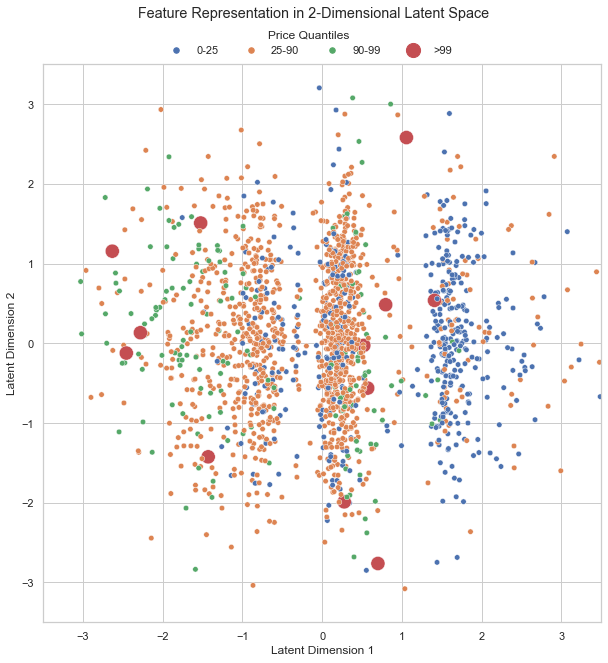
\includegraphics[width=0.8\textwidth]{latent_representation.png}
  \caption{Feature Representation in a two-dimensional latent space embedding}
  \label{fig:latent-representation}
\end{figure}
%%%

\Cref{fig:latent-representation} visualizes the two-dimensional feature embedding.
Already a \emph{single} dimension, here the horizontal axis, seems so be sufficient to categorize the observations into price ranges.
Cheaper apartments in blue are clustered on the right, medium prices in orange in the middle and higher prices in green are located on the left.

It is worth noting that the latent dimensions indeed \emph{combine} information from multiple features.
At the very beginning of our analysis we performed a bivariate analysis of each input feature and the response variable.
Since there was (by a large margin) no single variable with explanatory power comparable to the first latent dimension in \Cref{fig:latent-representation}, we can reject the hypothesis that the Encoder of the VAE simply maps original features of the data to the latent axes.

In contrast to the majority of listings, the top $1$\% of highest prices indicated by the large red circles do \emph{not} seem to build their own cluster, they are rather spread out across the entire feature space.
When the Network has to predict prices for some of the outliers in the \emph{center} of the latent space, they appear indistinguishable to their medium or even low-priced Nearest-Neighbours based on their feature set.
Hence, the network likely maps these outliers to comparably low price predictions resulting in large residuals with a high influence on the MAE and the $R^2$ value.

There are two possible explanations for this lack of separability in feature space with regards to the most expensive listings:

\begin{enumerate}
  \item The collected data is simply not rich or expressive enough to capture all factors that contribute to very high prices.
  \item Some apartments are listed at a price that does not represent their true value.
\end{enumerate}


The former reason illustrates why the outliers in the center of \Cref{fig:latent-representation} could still be worth their money:
There might exist unmeasured variables like historic or cultural significance of the building or a welcoming local community that are difficult to quantify appropriately and are not included in the feature set.

If the latter reason is predominant, it can be argued that the entire task of predicting Airbnb prices is questionable in the first place:
In order to draw connections from features to outputs, the process implicitly assumes observations whose listed price can be justified and explained by characteristics of the joint feature distribution.
If there is no connection between features and response in the first place, there is obviously no way for the model to recover this connection.

One question that needs to be addressed is why we are not simply removing the outliers completely prior to model fitting if they indicate such a large negative impact on the predictive performance.
As alluded to above, we have to distinguish between two groups of outliers:

\begin{enumerate}
  \item The first group contains expensive, but \emph{fairly priced} apartments.
        Those listings should be \emph{kept} in the data since it is very plausible that a new data set that our trained model is applied to contains such observations as well.
        To deliver useful results during inference, the model should have therefore learned to handle these cases appropriately during training.
  \item The second group consists of \emph{overpriced} listings that we would indeed like to remove from the data.
        However, it is actually very difficult to identify which observations exactly belong to this group.
        Potential candidates could be price outliers that indicate a very low demand since guests naturally try to maximize their cost-benefit ratio.
        Yet, it is entirely possible that few people want to pay that much money for \emph{any} apartment regardless of its true value, even if the price is actually justified.
\end{enumerate}

The differentiation between these two groups is nontrivial and remained a difficult problem throughout our analysis.


\subsection{Price Predictions on Munich Dataset}

To test the generalization ability of our implemented models, we applied them to the Airbnb data for \emph{Munich}, which is also published by the \emph{Inside Airbnb} project.
This data set includes roughly twice as many accommodations as the previous data set for Oslo.

\begin{table}[t]
  \centering
  \begin{tabular}{@{}ccc@{}}
    \toprule
    Quantile Threshold & MAE   & R2   \\ \midrule
    0.0                & 42.49 & 0.31 \\
    1.0                & 35.32 & 0.44 \\
    2.5                & 30.26 & 0.42 \\
    5.0                & 25.2  & 0.45 \\
    10.0               & 22.94 & 0.4  \\ \bottomrule
  \end{tabular}
  \caption{Mean Absolute Error and $R^2$ value of the Neural Network on the validation set after removing the highest quantiles of the price distribution from the Munich data set}
  \label{tab:munich-outliers}
\end{table}

As expected, the flexible models such as Gradient Boosting and the Neural Network benefit most from the larger number of observations.
The overall performance, however, is \emph{not} significantly better compared to the original Oslo data:
The Neural Net improved marginally from a MAE of $44.3$ Euros for Oslo to $42.5$ Euros for Munich on the validation set.
One exception was the Gradient Boosting Model that now shows by far the best test set performance with a MAE of $32.8$ Euros and a $R^2$ of $0.453$.
To further improve the Neural Network performance, a wider or deeper model architecture could be considered that is specifically designed for the larger data set.

Similar to Oslo, the most important predictors of the Munich data set were \emph{Property Type}, \emph{Neighborhood}, and \emph{Accommodates}.
Furthermore, the new data set also suffers from outliers whose influence is quantified in \Cref{tab:munich-outliers}.
Excluding consecutive percentiles of the price distribution prior to fitting the model again leads to a significant improvements in MAE and $R^2$.
In contrast to Oslo, however, we can not detect a huge jump from using the entire data to cutting off the top $1$\% of highest prices.









